% intensity
% spectral distribution
% solar geometry
% saules stāvoklis debesīs
% un virziens, kurā stara starojums krīt uz dažādu virzienu un ēnojuma virsmām

\section{Saules apstarojums}

Lielākā daļa Saules emitētās enerģijas tiek saražota kodolreakcijās fotosfērā.

% Saņemto enerģiju laika vienībā uz uz laukuma vienības perpendikulāri starojuma izplatīšanās virzienam 1 AU attālumā integrēta pa visiem viļņu garumiem raksturo solārā konstante ($G_{sc}$).

Solārā konstante $G_{sc}$ ir saņemtā enerģija laika vienībā uz laukuma vienības perpendikulāri starojuma izplatīšanās virzienam 1 AU attālumā integrēta pa visiem viļņu garumiem.\cite{ThermalProcesses}

Kopējā saules apstarojuma vērtība mainās laikā un korelē ar Saules plankumu ciklu.
Viena fizikālā lieluma tikai daļēji pārklājušos novērojumu laikrindu apvienošana kompozītā ir gan zinātnisks, gan statistisks izaicinājums un neviens kompozīts (piemēram, PMOD, ACRIM, IRBM) līdz šim nav guvis konsensu solārā apstarojuma pētnieku kopienā.~\ref{fig:TSI_misijas}

Par labāko saules apstarojuma mērījumu reprezentāciju tiek uzskatīti TIM instrumenta dati mēraparāta uzbūves (TIM ir lielāka precizitātes apertūra tuvu dobumam un mazāka redzeslauku bloķējošā pie instrumenta ieejas, klasiskajos radiometros ir pretēji, kas palielina jutību pret atstaroto gaismu no redzeslauku bloķējošās apertūras un kļūdu no instrumenta sasildīšanas) un augstās precizitātes dēļ, tāpēc šajā darbā grafiki balstās uz šiem mērījumiem, pēc kuriem absolūtā kopējā saules apstarojuma vērtība ir $1360.8 \pm 0.5 \textrm{Wm}^{-2}$.\cite{Frohlich2012}

\begin{figure}[h]
    \centering
    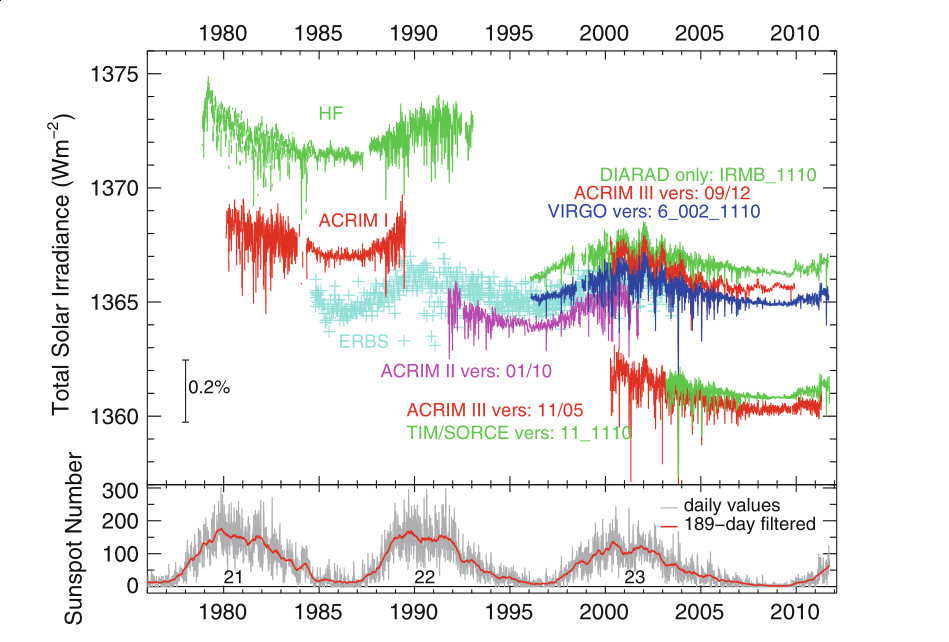
\includegraphics[width=0.6\linewidth]{figures/misc/TSI_misijas.png}
    \caption{Salīdzinājums dienā vidējotiem saules kopējā apstarojuma datiem no dažādām misijām un Saules plankuma skaitlis, lai ilustrētu solārās aktivitātes variabilitāti trīs ciklos. \cite{Frohlich2012}}
    \label{fig:TSI_misijas}
\end{figure}

\begin{table}[h]
    \caption{TSI mērījumu vēsture} % caption iet pirms tabulas
    \begin{center}
    \begin{tabular}{| r | c | l |}
    \hline
    radiometrs & misija & darbības laiks \\ \hline
    Hickey-Frieden & NIMBUS-7 & 1978--1992  \\ \hline
	ACRIM I & Solārā Maksimuma Misija (SMM) & 1980--1989 \\ \hline
	ACRIM  & Zemes Radiācijas Budžeta Satelīts (ERBS) & 1984--2003 \\ \hline
	ACRIM II & Augšējās Atmosfēras Izpētes Satelīts (UARS) & 1991--2001 \\ \hline
	VIRGO & Solārā un Heliosfēras observatorija (SOHO)& 1996--pašlaik \\ \hline
	ACRIM III & ACRIMSAT  & 2000--pašlaik \\ \hline
	TIM & Saules Radiācijas un Klimata Eksperiments (SORCE) & 2003--pašlaik\\ \hline
    \end{tabular}
    \end{center}
    \label{tab:radiometers}
\end{table}


% Kopējais saules apstarojums (TSI) ir saules starojuma absolūtās intensitātes mērījums integrēts visā saules enerģijas diskā un visā saules enerģijas spektrā.
% diennakts vidējais apstarojums 1 AU attālumā no Saules.
% Norāda uz solārās radiācijas izmaiņām, kas ietekmē solārās enerģijas apjomu uz Zemes atmosfēras augšējiem slāņiem.


\begin{figure}[h]
    \centering
    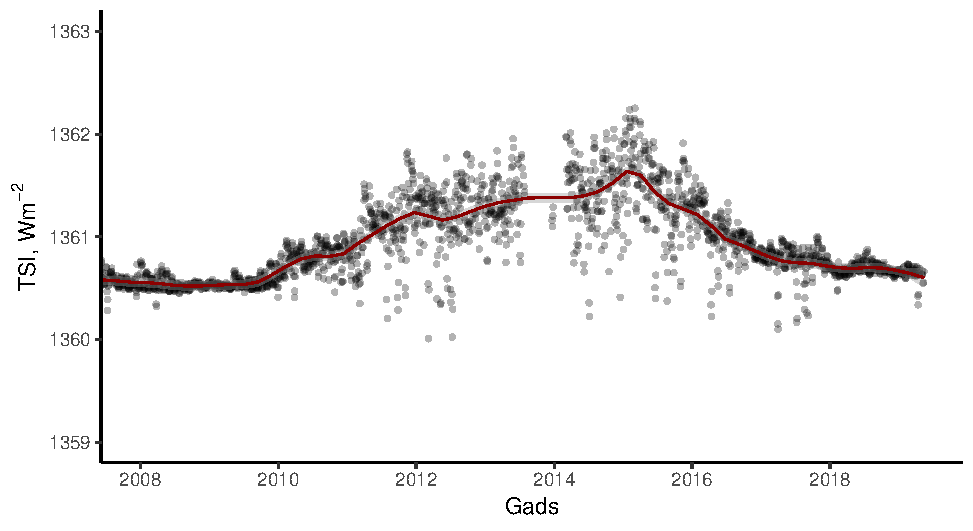
\includegraphics[width=\linewidth]{figures/misc/TSI_8-19.pdf}
    \caption{Kopējais saules apstarojums 24. saules ciklā \cite{TSIdata}}
    \label{fig:TSI1}
\end{figure}

\begin{figure}[h]
    \centering
    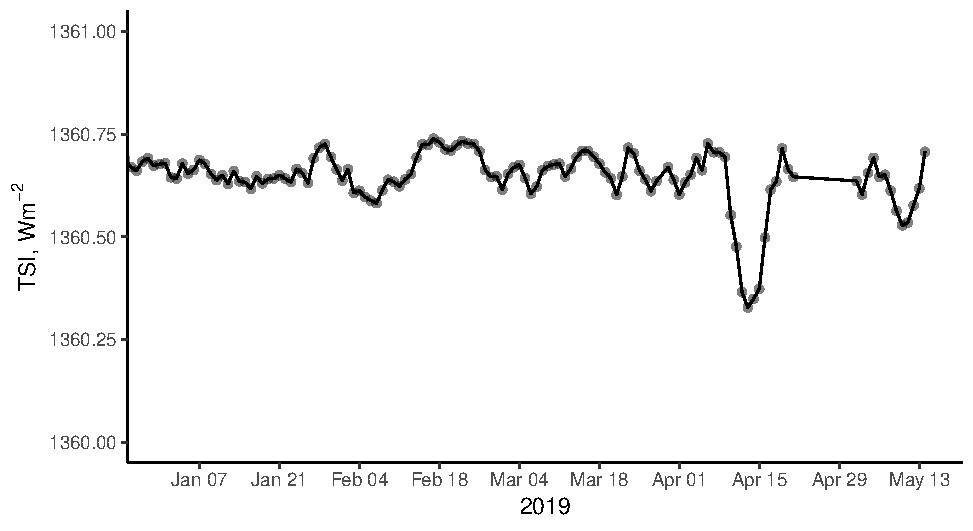
\includegraphics[width=\linewidth]{figures/misc/TSI.pdf}
    \caption{Kopējais saules apstarojums solāro paneļu datu ieguves laikā \cite{TSIdata}}
    \label{fig:TSI2}
\end{figure}

\begin{figure}[h]
    \centering
    \includegraphics[width=\linewidth]{figures/misc/LV_DNI.png}
    \caption{Tiešais normālais apstarojums \cite{solargis}}
    \label{fig:lv_DNI}
\end{figure}
\begin{figure}[h]
    \centering
    \includegraphics[width=\linewidth]{figures/misc/LV_GHI.png}
    \caption{Globālais horizontālais apstarojums Latvijā \cite{solargis}}
    \label{fig:lv_GHI}
\end{figure}
\begin{figure}[h]
    \centering
    \includegraphics[width=\linewidth]{figures/misc/LV_PVOUT.png}
    \caption{PV potenciālā jauda \cite{solargis}}
    \label{fig:lv_PVOUT}
\end{figure}
